\chapter{The influence of the group environment}


\section{Group Identification}\label{sec:groups}

We used the \citet{berlind06} catalogue, which uses a friends-of-friends algorithm to identify group and cluster galaxies in the SDSS. This was cross matched to the \textsc{gz-galex} sample and limited to $z < 0.1$ to ensure GALEX completeness of the red sequence (see \citealt{ref}). Centrals were selected as the brightest galaxy in a group and all others were designated as satellites. This resulted in a sample of $14,199$ group galaxies with $3,468$ centrals and $10,731$ satellites within a projected cluster centric radius range of $0 < R/R_{200} < 25$ and $z < 0.084$. 

In this work we focus on galaxies which are either quenching or quenched and are more than $\pm1\sigma$ below the star forming `main sequence'. This encompasses $4629$ satellite and $2314$ central galaxies and will be referred to as the \textsc{gz-group} sample. {\notebsm These galaxies are highlighted in red on Figure \ref{}. }

\subsection{Field sample}\label{sec:field}

For all galaxies in the \textsc{gz-galex} sample, we calculated the smallest projected cluster centric radii from each of the central galaxies in the  \citet{berlind06} catalog and selected candidate field galaxies as those with (i) $R/R_{200} > 25$ and (ii) $\log\Sigma < -0.8$ from \cite{baldry06}. This sample of field galaxy candidates was then matched in redshift and stellar mass firstly to the central galaxies of the \textsc{gz-group} sample to give $2,309$ field galaxies with $z < 0.084$ which will be referred to as the \textsc{gz-cent-field} sample. Secondly, the field galaxy candidates were then matched in redshift and stellar mass to the satellite galaxies of the \textsc{gz-group} sample to give $6,849$ field galaxies with $z < 0.084$ which will be referred to as the \textsc{gz-sat-field}. These galaxies in the \textsc{gz-sat-field} sample will be used as a control when investigating the morphological trends of satellite galaxies with environment. 

As in Section \ref{sec:groups} we select all those galaxies in the central matched sample $\pm1\sigma$ below the star forming `main sequence', giving $1596$ quenching or quenched field galaxies for use as a control sample, which will be referred to as the \textsc{gz-cent-field-q} sample. These galaxies will be used as a control when investigating the quenching parameters of the different environments in order to ensure that each galaxy under comparison resides in similar stellar mass halos. 
%We also select all those galaxies in the satellite matched sample $\pm1\sigma$ below the star forming `main sequence', giving $$ quenching or quenched field galaxies for use as a control sample, which will be referred to as the \textsc{gz-sat-field-q} sample.
  
\begin{figure*}
\centering{
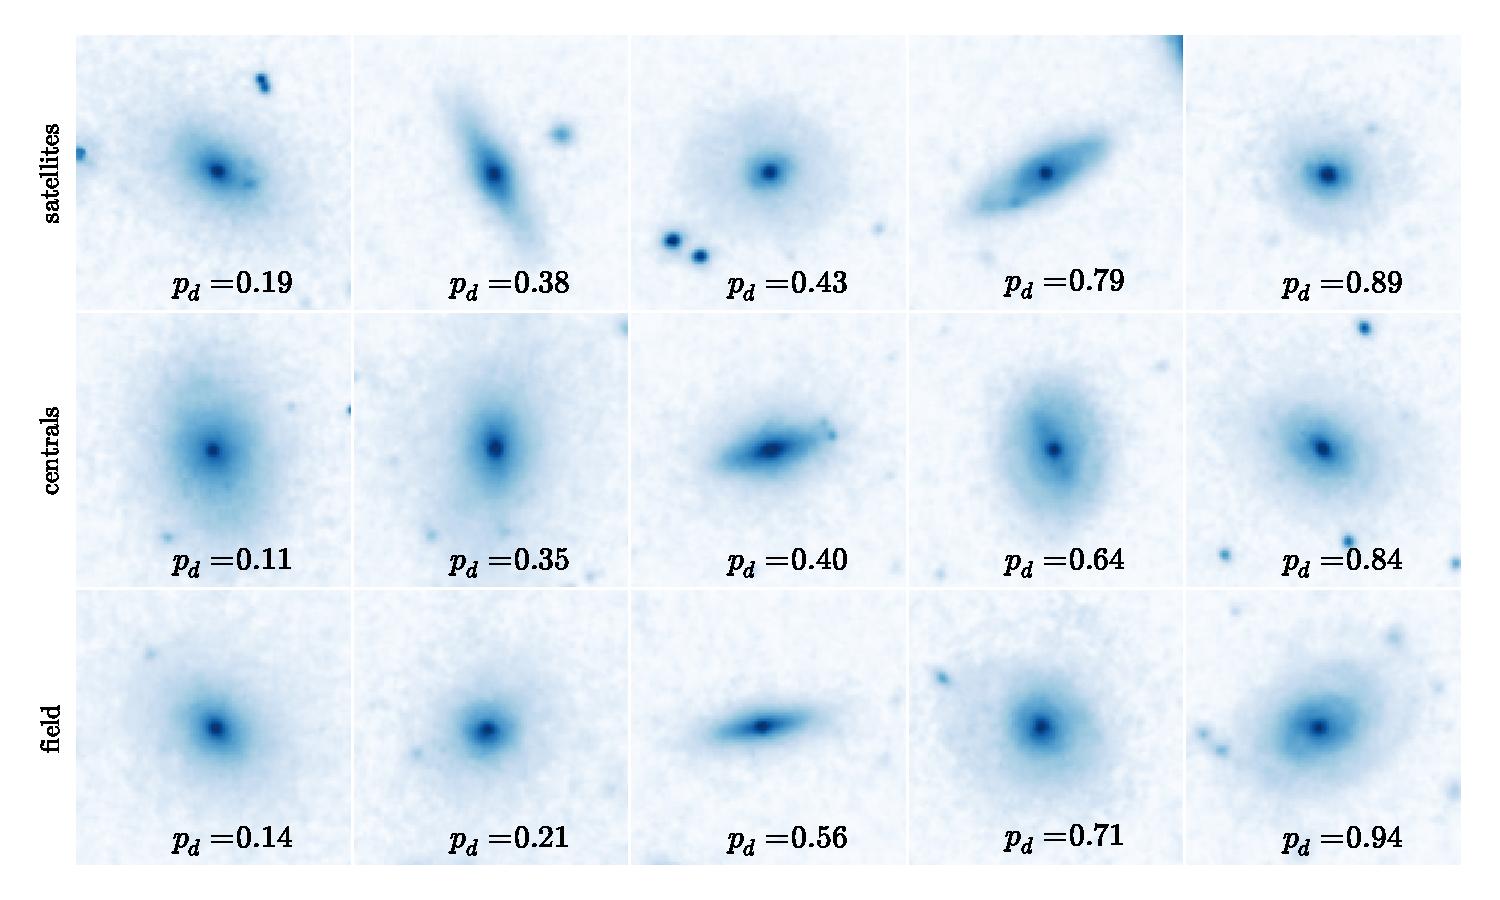
\includegraphics[width=0.95\textwidth]{environment/mosaic_sat_cent_field_disc_fraction.pdf}
\caption[SDSS images of galaxies in the \textsc{gz-group} and  \textsc{gz-field} samples]{Randomly selected SDSS \emph{gri} composite images of satellite and central galaxies in the \textsc{gz-group} sample in comparison to those from the \textsc{gz-field} sample. All galaxies lie within $0.04 < z < 0.05$ and in the central galaxy mass range $10^{10.5} < M_{*} [M_{\odot}] < 10^{11}$, used as a proxy for halo mass. The galaxies are ordered from least to most featured according to their debiased `disc or featured' vote fraction, $p_d$ (see \citealt{GZ2}). The scale for each image is $0.099~\rm{arcsec/pixel}$.}}
\label{fig:mosaic}
\end{figure*}

\begin{figure}
\centering{
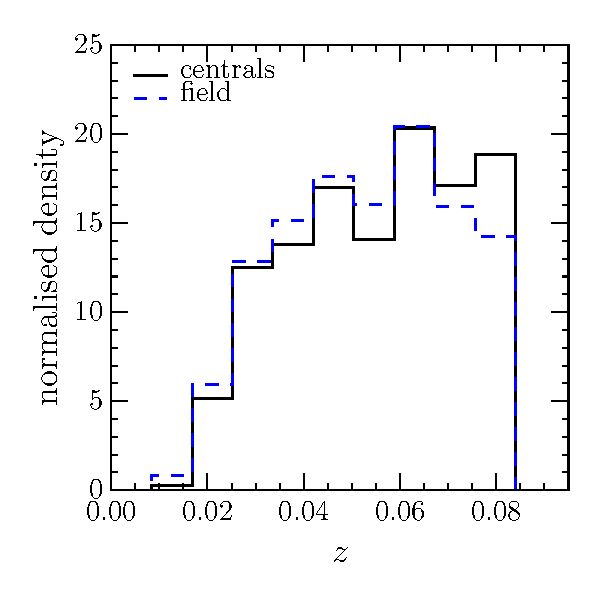
\includegraphics[width=0.8\textwidth]{environment/redshift_cent_field.pdf}
\caption[Redshift distribution comparison of the \textsc{gz-group} sample and matched control \textsc{gz-cent-field-q} sample]{Redshift distributions of quenching or quenched central galaxies in the \textsc{gz-group} sample (black solid line) in comparison to the redshift and mass matched \textsc{gz-cent-field-q} sample (blue dashed line).}}
\label{fig:zcompare}
\end{figure}

\section{Results}\label{sec:results}

\begin{figure}
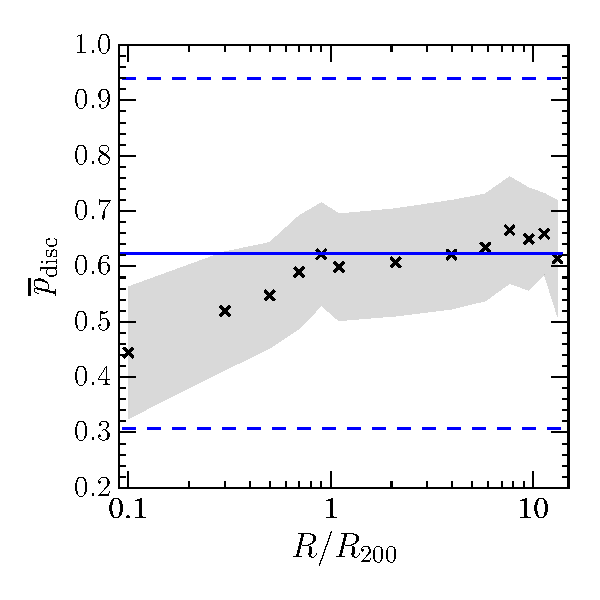
\includegraphics[width=0.46\textwidth]{environment/p_disc_trend_with_log_radius_field_compare.pdf}
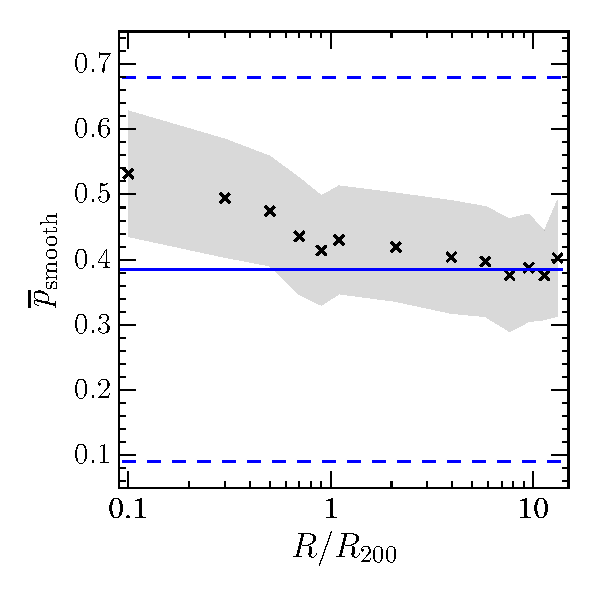
\includegraphics[width=0.46\textwidth]{environment/p_smooth_trend_with_log_radius_field_compare.pdf}
\caption[Mean GZ vote fractions for satellite galaxies with projected cluster centric radius]{Mean GZ vote fraction for disc (top) and smooth (bottom) galaxies in the \textsc{gz-group} sample binned in projected cluster centric radius, normalised by $R_{200}$, a proxy for the virial radius of a group. The shaded region shows $\pm1\sigma$ on the mean vote fraction. The mean vote fraction of the \textsc{field} sample are also shown (blue solid lines) with $\pm1\sigma$ (blue dashed lines).}
\label{fig:morphradius}
\end{figure}

\begin{figure}
\centering{
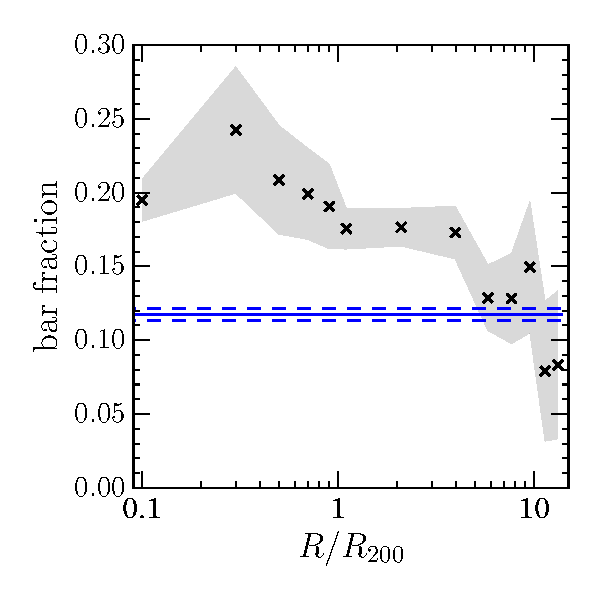
\includegraphics[width=0.95\textwidth]{environment/bar_fraction_over_disc_trend_with_log_radius_sat_matched_field_cand.pdf}
\caption[Bar fraction of satellite disc galaxies with projected cluster centric radius]{Bar fraction (number of barred disc galaxies over number of disc galaxies) in the \textsc{gz-group} sample binned in projected cluster centric radius, normalised by $R_{200}$, a proxy for the virial radius of a group. The shaded region shows $\pm1\sigma$ on the bar fraction. The bar fraction of the \textsc{gz-sat-field} sample is also shown (blue solid line) with $\pm1\sigma$ (blue dashed line).}}
\label{fig:barradius}
\end{figure}

\begin{figure}
\centering{
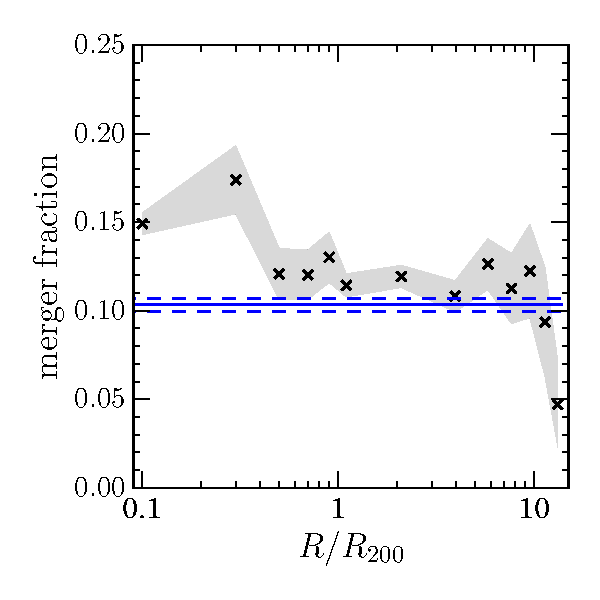
\includegraphics[width=0.95\textwidth]{environment/merger_fraction_trend_with_log_radius_compare_sat_field_cand.pdf}
\caption[Merger fraction of satellite galaxies with projected cluster centric radius]{Merger fraction in the \textsc{gz-group} sample binned in projected cluster centric radius, normalised by $R_{200}$, a proxy for the virial radius of a group. The shaded region shows $\pm1\sigma$ on the merger fraction. The merger fraction of the \textsc{gz-sat-field} sample is also shown (blue solid line) with $\pm1\sigma$ (blue dashed line).}}
\label{fig:mergerradius}
\end{figure}

First start with a sanity check - do we reproduce morphology-density relation of \citealt{dressler80}? Figure \ref{fig:morphradius} shows the mean disc and smooth vote fractions from galaxy zoo, binned in projected cluster centric radius (normalised by the approximate viral radius of each group, $R_{200}$). We can see that the mean disc (smooth) vote fraction decreases (increases) from the mean field value (blue line) past $1$ virial radius.

Figure \ref{fig:barradius} shows how the bar fraction (number of barred disc galaxies over the number of disc galaxies) increases towards the centre of the group population suggesting the possibility that the environment may play a role in triggering the disk instabilities which produce a morphological bar \citep{ref, ref, ref}. 

Figure \ref{fig:mergerradius} shows how the merger fraction does not significantly deviate from the field fraction (blue line) until beyond $1$ virial radius. Similarly in Figure \ref{fig:bulgeradius} the left panel shows how those galaxies identified as having no or just noticeable bulges are less common in the inner regions of the cluster (left panel), whereas the fraction of galaxies with obvious or dominant bulges (thought to be grown by mergers;\citealt{ref, ref, ref}) increases with decreasing projected distance from the centre of the cluster 

Figure \ref{fig:sfrradius} shows how the SFR of the \textsc{gz-group} sample declines with decreasing cluster centric distance, significantly below the mean SFR of the \textsc{gz-field} sample shown by the blue dashed line. This is in agreement with the results of \cite{gomez03} who observe the decline in SFR with cluster centric radius in SDSS clusters (see for example, Figure 6 in \citealt{gomez03}). 

With the results from \starpy~ we can look at the time since quenching onset ($\Delta t = t_{obs} - t_{q}$, see Section \ref{}) binned in projected cluster centric radius, normalised by $R_{200}$ (a proxy for virial radius) for satellite galaxies and central galaxies in the \textsc{gz-group} sample, compared with galaxies in the \textsc{gz-field} sample. We can investigate these trends with group properties as shown in Figures \ref{fig:timesinceradius} \& \ref{fig:timesinceradiusvel}. 

If mergers are an important evolutionary mechanism for satellite galaxies, we expect to see a difference in the quenching histories of satellites in groups with a higher number of galaxies, $N_{group}$. However, if we look at the bottom panel of Figure \ref{fig:timesinceradius} we do not see a trend with time since quenching onset with increasing $N_{group}$ for the satellite galaxies. The only place we do see such a trend for the central galaxies. 

Across all the panels in Figures \ref{fig:timesinceradius} \& \ref{fig:timesinceradiusvel} we see a general trend for increasing time since quench with decreasing distance from the centre, which is suggestive that this slight trend is due to an effect of the environment itself. As earlier, in Figures \ref{fig:morphradius}$-$\ref{fig:bulgeradius} significant differences from the field value arise beyond approximately one virial radius. 

In the middle panel of Figure \ref{fig:timesinceradius} however, we do see a clear trend for increasing time since quenching onset with increasing stellar mass for both satellite and central galaxies. This is suggestive of mass quenching among the group galaxy population. This is contrary to previous work suggesting that mass quenching is only of import for central galaxies \citep{ref, ref, ref}. 

In simulations, the three things that are seen to constrain galaxy evolution are redshift, mass and halo mass \cite{ref, ref}. To study the effect that halo mass has on the quenching properties of group galaxies we shall use a proxy for halo mass by splitting by the mass of the corresponding central galaxy of the group.

We investigate the effect of the group halo mass in the top panel of Figure \ref{fig:timesinceradius} where we can once again see a clear trend for increasing time since quenching onset with increasing stellar mass of the group central for both satellite and central galaxies. More massive halos therefore have a greater impact on the star formation rate of their satellites than less massive halos. 

In the bottom panel of Figure \ref{fig:timesinceradiusvel} we split the satellite galaxies of the \textsc{gz-group} sample into bins of relative velocity to their central galaxies. We can see that their is no trend with time since onset of quenching with increasing relative velocity for satellite galaxies, however the trend with decreasing projected group centric radius, seen in each panel in Figure \ref{fig:timesinceradius} is still present. This suggests that any environmental processes causing this quenching are not corrected with satellite velocity.  

\begin{figure*}
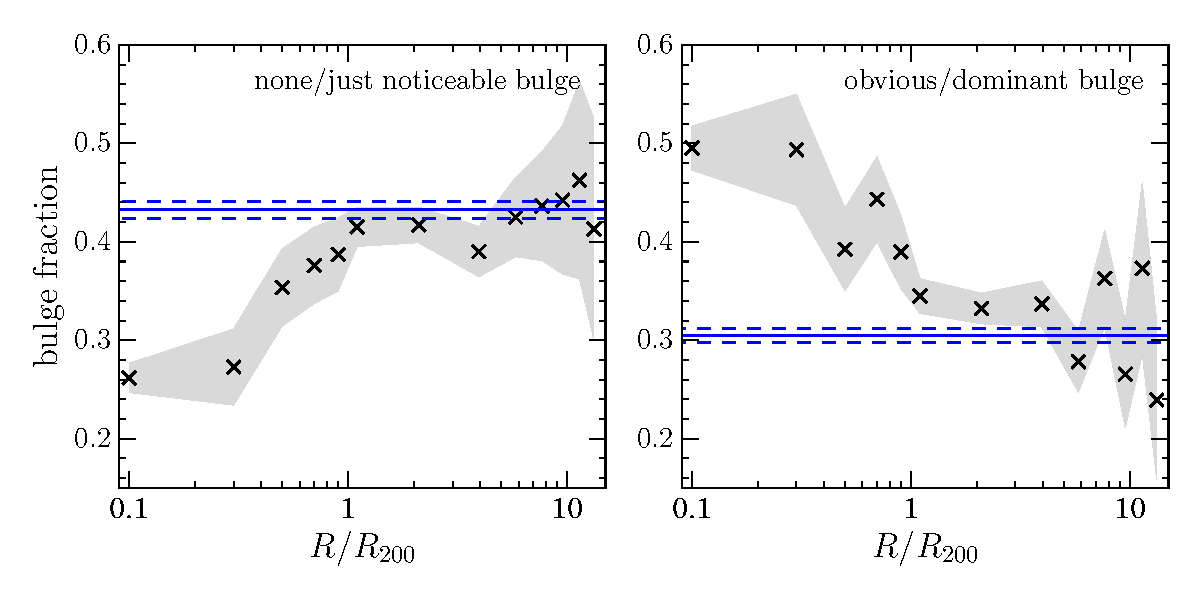
\includegraphics[width=\textwidth]{environment/min_max_bulge_fraction_trend_with_log_radius_sat_field_cand.pdf}
\caption[GZ2 bulge fractions of satellite disc galaxies with projected cluster centric radius]{Fraction of galaxies with none/just noticeable bulge classifications (left) and with obvious/dominant bulge classifications (right) in the \textsc{gz-group} sample binned in projected cluster centric radius, normalised by $R_{200}$, a proxy for the virial radius of a group. The shaded regions shows $\pm1\sigma$ on the bulge fractions. The bulge fractions of the \textsc{gz-sat-field} sample are also shown (blue solid lines) with $\pm1\sigma$ (blue dashed lines).}
\label{fig:bulgeradius}
\end{figure*}

\begin{figure}
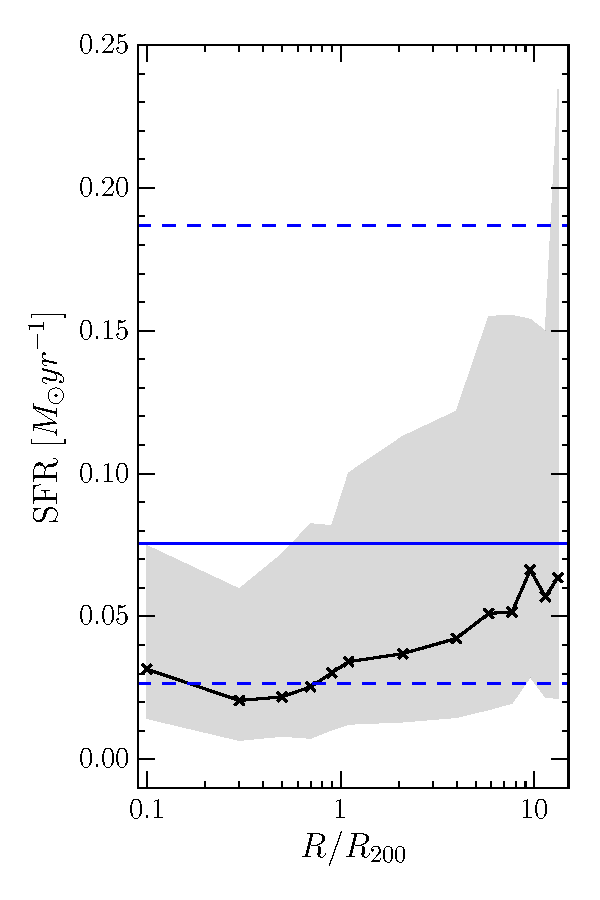
\includegraphics[height=0.825\textheight]{environment/sfr_trend_with_log_radius_field_matched_blue_dashed_hlines_gomez_03_rv_not_r200.pdf}
\caption[Median SFR of the \textsc{gz-group} sample with projected cluster centric radius]{Median $H\alpha$ derived star formation rates of satellite galaxies in the \textsc{gz-group} sample, binned in projected cluster centric radius, normalised by $R_{200}$, a proxy for the virial radius of a group.  The shaded region shows the SFRs encompassed by $50\%$ of the population in a given bin. The median SFR of the \textsc{gz-sat-field} sample is shown (blue solid line) along with the 25th and 75th percentiles (blue dashed lines).}
\label{fig:sfrradius}
\end{figure}

\begin{figure}
\centering{
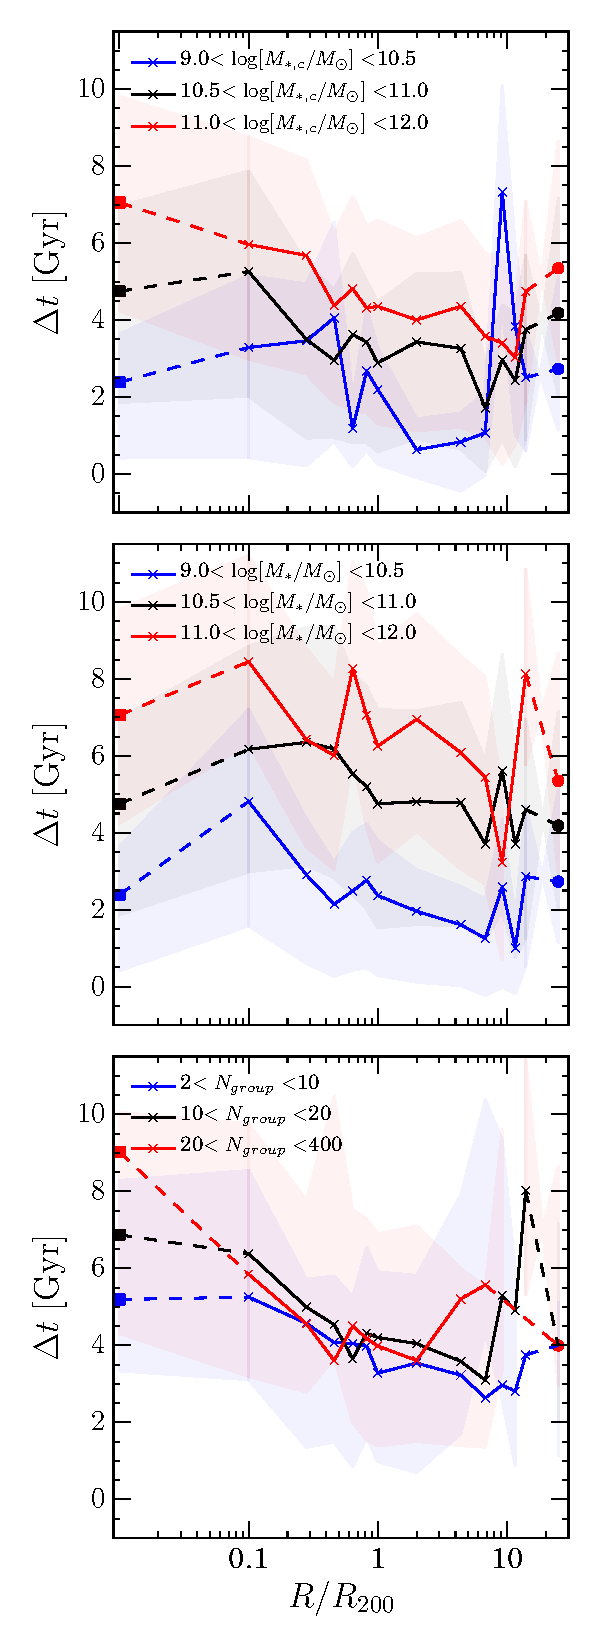
\includegraphics[height=0.825\textheight]{environment/time_since_quenching_environment_properties.pdf}
\caption[The time since quenching of the \textsc{gz-group} sample with projected cluster centric radius]{The time since quenching onset ($\Delta t = t_{obs} - t_{q}$) binned in projected cluster centric radius, normalised by $R_{200}$, for satellite galaxies (triangles) split by stellar mass of the corresponding central galaxy (top), stellar mass (middle) and the number of galaxies within the group (bottom). The corresponding values for central galaxies (squares) and galaxies in the \textsc{gz-cent-field} sample (circles) are shown and connected by the dashed lines to aid the reader.}
\label{fig:timesinceradius}}
\end{figure}

\begin{figure}
\centering{
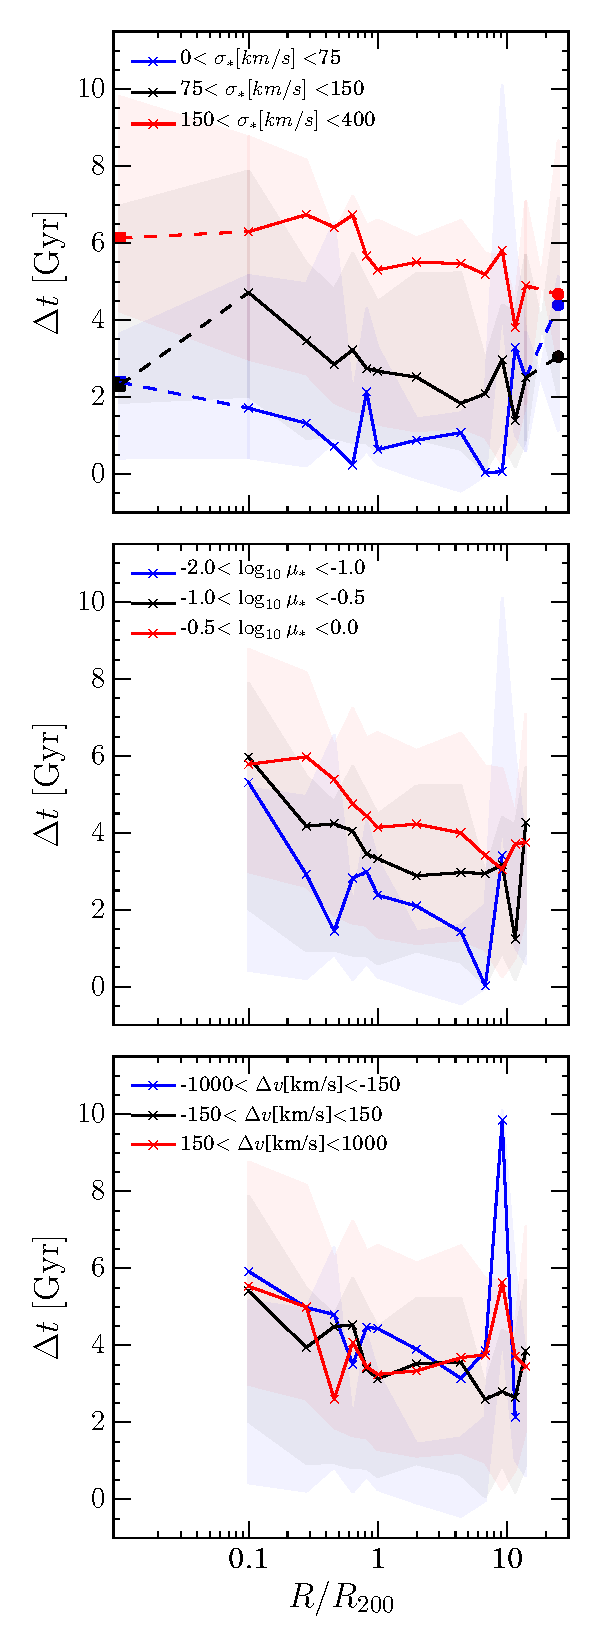
\includegraphics[height=0.825\textheight]{environment/time_since_quenching_v_disp_mu_bins_delv.pdf}
\caption[The time since quenching of the \textsc{gz-group} sample with projected cluster centric radius]{The time since quenching onset ($\Delta t = t_{obs} - t_{q}$) binned in projected cluster centric radius, normalised by $R_{200}$, for satellite galaxies (triangles) split by velocity dispersion (top), stellar mass ratio ($\mu_* = M_*/M_{*,c}$) (middle) and the difference in velocity from the associated central galaxy (bottom). The corresponding values for central galaxies (squares) and galaxies in the \textsc{gz-cent-field} sample (circles) are shown and connected by the dashed lines to aid the reader in the top panel where appropriate.}
\label{fig:timesinceradiusvel}}
\end{figure}


\section{Discussion}\label{sec:disc}

We have shown that mergers are important for centrals not for satellites in the bottom panel of Figure \ref{fig:timesinceradius}, that mass quenching is important for satellites as well as centrals in the middle panel of Figure \ref{fig:timesinceradius} and that larger halos have a stronger environmental effect on their satellites in the top panel of Figure \ref{fig:timesinceradius}. 

The trend that is present in all panels of Figure \ref{fig:timesinceradius} was for increasing time since quenching onset with decreasing projected group centric distance. We argue that this lends more support for quenching caused directly by the environmental; galaxies closer in, fell into the group earlier, as they did so they started quenching and so have a longer time since quenching started to occur. However, as seen in Figure \ref{fig:timesinceradiusvel} there is no trend in the time since quenching onset with the relative velocity of the satellites to their corresponding central. This suggests that whatever environmental mechanism is at play here, it is dependant on the size of the halo, either due to the potential or temperature of the halo, but not dependant on the speed of the satellite as in ram pressure stripping theory. This suggests that ram pressure stripping is not the dominant environmental quenching mechanism. 
